\documentclass{standalone}
\usepackage{tikz}
\usetikzlibrary{positioning,arrows}
\begin{document}
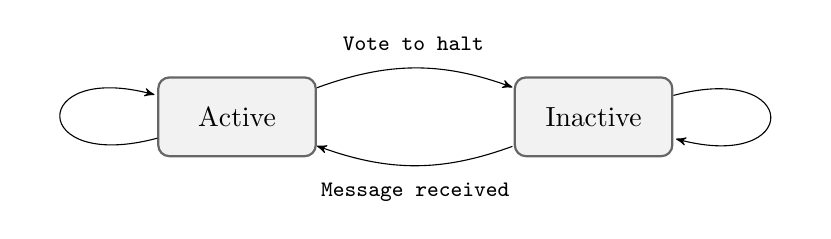
\begin{tikzpicture}[
        state/.style={
                rectangle,
                rounded corners,
                draw=black!60,
                fill=black!5,
                thick,
                minimum width=20mm,
                minimum height=10mm
            },
        predicate/.style = {font=\footnotesize\ttfamily},
        >=stealth',
        shorten >=0.5pt
    ]
    \node[state] (active) {Active};
    \node[state] (inactive) [right=2.5cm of active] {Inactive};

    \path[->,in=180-20,out=0+20] (active) edge node[predicate,above=1mm,pos=.49] {Vote to halt} (inactive);
    \path[<-,in=180+20,out=0-20] (active) edge node[predicate,below=1mm] {Message received} (inactive);
    \path[->] (active)   edge[loop left]  node {} (active);
    \path[->] (inactive) edge[loop right] node {} (inactive);
\end{tikzpicture}
\end{document}